\subsection{Software architectuur}
\label{subsecion:SoftwareArhitectuur}
Om de onderhoudbaarheid te verbeteren van het huidige CMS is er ook nagedacht over het opzetten van de code.
Hiervoor is er gekeken hoe de architectuur zich houdt aan de verschillende SOLID principes \parencite{SOLID}. 
SOLID is een acroniem dat 5 verschillende principes inhoudt.
Deze principes zorgen ervoor dat de code beter te onderhoudbaar is en makkelijker te begrijpen is.
SOLID bestaat uit de volgende principes:

\begin{enumerate}
    \item \textbf{Single-responsibility principle}
    Dit betekent dat een class\slash module, maar 1 verantwoordelijk mag hebben.
    Als een class\slash module te veel verantwoordelijkheden heeft dan wordt het moeilijker om de code te begrijpen en aan te passen.

    \item \textbf{Open-closed principle}
    Dit houdt in als class of functie of een andere software entiteit uitgebreid moet worden dat het wordt gedaan door middel van een extentie(open) in plaats van modificatie(closed).
    Hierdoor hou je oude code intact en heb je geen risico dat je bestaande code stuk gaat vanwege de nieuwe functionaliteit die geschreven is. 
        
    \item \textbf{Liskov substitution principle}
    Een class die afgeleid is van een super class zou moeten vervangen kunnen worden van een andere afgeleiden variant van die superclass
    Dit moet gedaan kunnen worden zonder de validiteit (corectness) van het programma te beïnvloeden.
    Door het gebruik van het Liskov substitution principle verhoog je de consistentiteit en de verwachte uitkomst van je programma.

    \item \textbf{Interface segregation} 
    Een interface moet alleen de methods geven die nodig is voor de client. 
    Geen client moet geforceerd zijn om methodes te implementeren waar die geen gebruik van maakt.
    Dit kan verminderd worden om meerdere kleinere interfaces te maken inplaatst van een grote interface.
    Deze interfaces zijn verantwoordelijk voor meer specifieke usecases in plaats van generaliseerde usecases

    \item \textbf{Dependency inversion} 
    Een class of module zou niet moeten afhangen van implementaties maar van abstracties.
    Hierdoor verminder je de koppeling van de modules/classes, en verhoog je de code onderhoudbaarheid.
    Om aan dit principe te voldoen wordt er vaak gebruik gemaakt van dependency injection.
\end{enumerate}

\whitespace
Om de verschillende aspecten van SOLID te implementeren is er gekozen om gebruik te maken van handlers.
Hierbij heeft elke handler één taak.
Daarnaast wordt er ook gebruikgemaakt van een repository pattern om met de database te communiceren.
Er is gekozen om gebruik te maken van een repository pattern zodat er geen afhankelijkheid is van de database.
Een sequencediagram van deze architectuur is te zien in figuur \ref{fig:SequenceDiagramHandlerStructure}

\begin{graphic}
    \captionsetup{type=figure}
    \caption{Sequencediagram Handler structuur}
    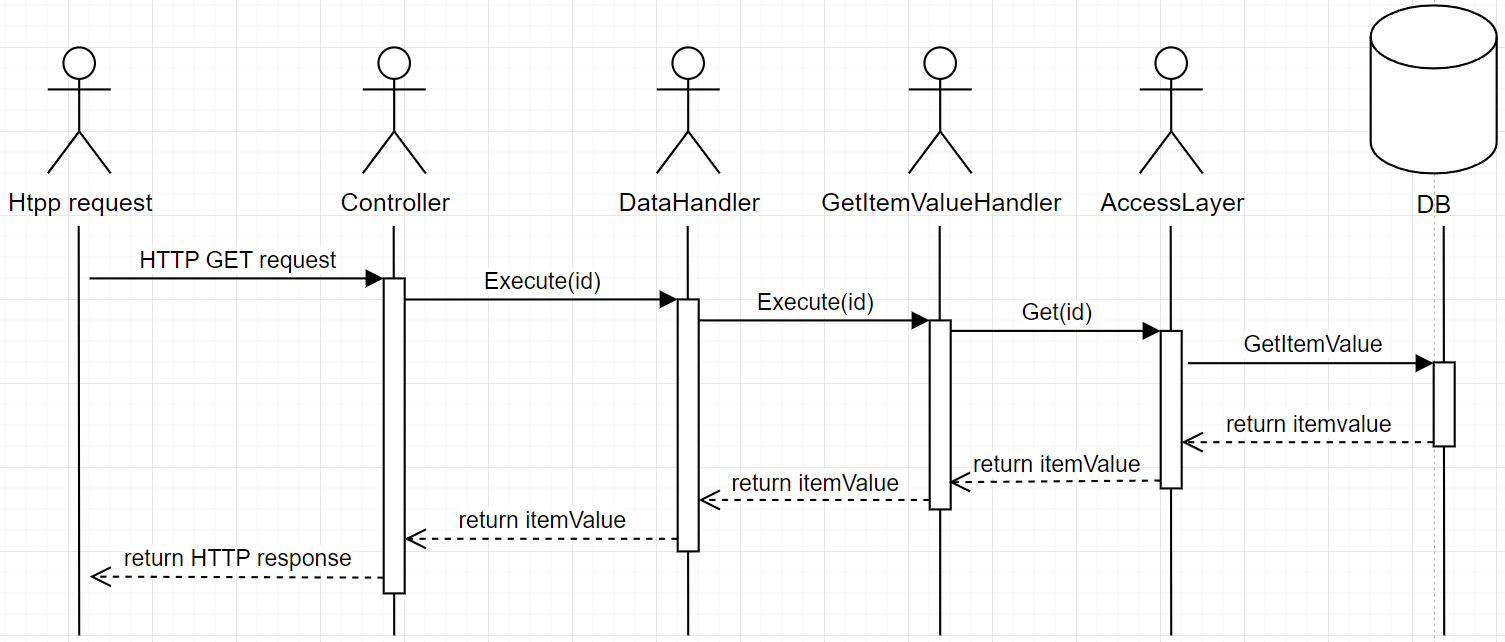
\includegraphics[scale=0.4]{SequenceDiagramArchitectureStructure.png}
    \label{fig:SequenceDiagramHandlerStructure}
\end{graphic}

\whitespace
De verschillende handlers zorgen ervoor dat het single-responsibility principle na gevolgd wordt.
Omdat elke handler maar 1 verantwoordelijk heeft.
Verder worden er kleine interfaces gebruikt om aan het Interface segregation principle te volgen.
En als laatste worden de verschillende dependencies geïnjecteerd (dependency injection pattern) om harde koppeling te voorkomen.
